\documentclass[14pt]{extbook}
\usepackage{multicol, enumerate, enumitem, hyperref, color, soul, setspace, parskip, fancyhdr} %General Packages
\usepackage{amssymb, amsthm, amsmath, bbm, latexsym, units, mathtools} %Math Packages
\everymath{\displaystyle} %All math in Display Style
% Packages with additional options
\usepackage[headsep=0.5cm,headheight=12pt, left=1 in,right= 1 in,top= 1 in,bottom= 1 in]{geometry}
\usepackage[usenames,dvipsnames]{xcolor}
\usepackage{dashrule}  % Package to use the command below to create lines between items
\newcommand{\litem}[1]{\item#1\hspace*{-1cm}\rule{\textwidth}{0.4pt}}
\pagestyle{fancy}
\lhead{Progress Quiz 9}
\chead{}
\rhead{Version A}
\lfoot{8590-6105}
\cfoot{}
\rfoot{Fall 2020}
\begin{document}

\begin{enumerate}
\litem{
Solve the radical equation below. Then, choose the interval(s) that the solution(s) belongs to.\[ \sqrt{-9 x - 3} - \sqrt{-7 x - 5} = 0 \]\begin{enumerate}[label=\Alph*.]
\item \( x_1 \in [-1.1, -0.39] \text{ and } x_2 \in [-0.9,0.08] \)
\item \( x \in [0.84,1.45] \)
\item \( x_1 \in [-0.48, 0.13] \text{ and } x_2 \in [0.42,1.28] \)
\item \( x \in [-4.15,-3.84] \)
\item \( \text{All solutions lead to invalid or complex values in the equation.} \)

\end{enumerate} }
\litem{
Solve the radical equation below. Then, choose the interval(s) that the solution(s) belongs to.\[ \sqrt{-8 x^2 - 25} - \sqrt{-30 x} = 0 \]\begin{enumerate}[label=\Alph*.]
\item \( x_1 \in [0.5, 1.5] \text{ and } x_2 \in [2.5,7.5] \)
\item \( \text{All solutions lead to invalid or complex values in the equation.} \)
\item \( x_1 \in [-2.6, 0.8] \text{ and } x_2 \in [-6.5,0.5] \)
\item \( x \in [0.5,1.5] \)
\item \( x \in [1.3,2.7] \)

\end{enumerate} }
\litem{
Choose the graph of the equation below.\[ f(x) = - \sqrt{x - 6} + 3 \]\begin{enumerate}[label=\Alph*.]
\begin{multicols}{2}\item 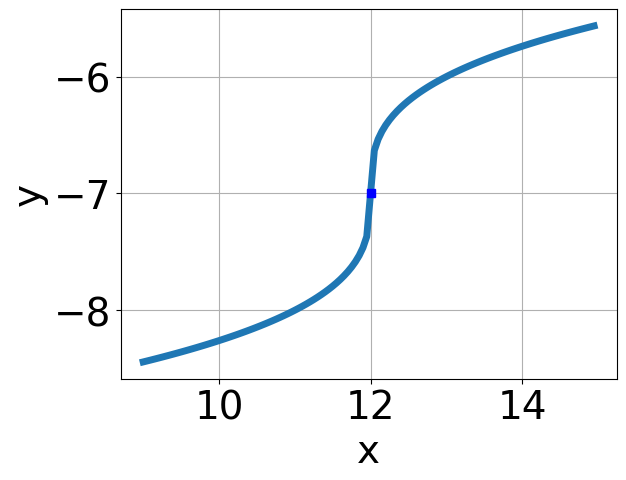
\includegraphics[width = 0.3\textwidth]{../Figures/radicalEquationToGraphAA.png}\item 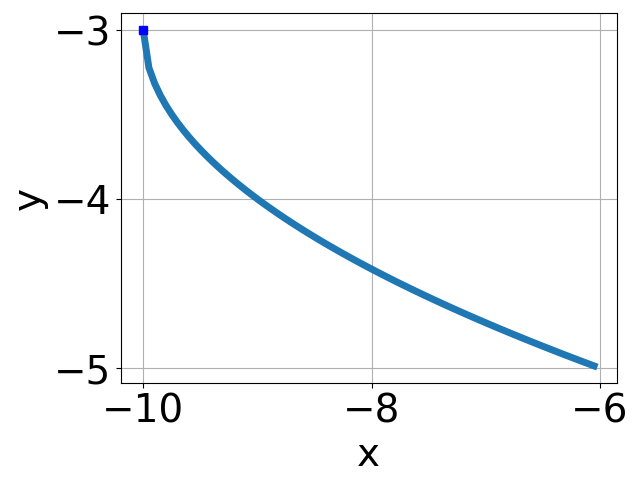
\includegraphics[width = 0.3\textwidth]{../Figures/radicalEquationToGraphBA.png}\item 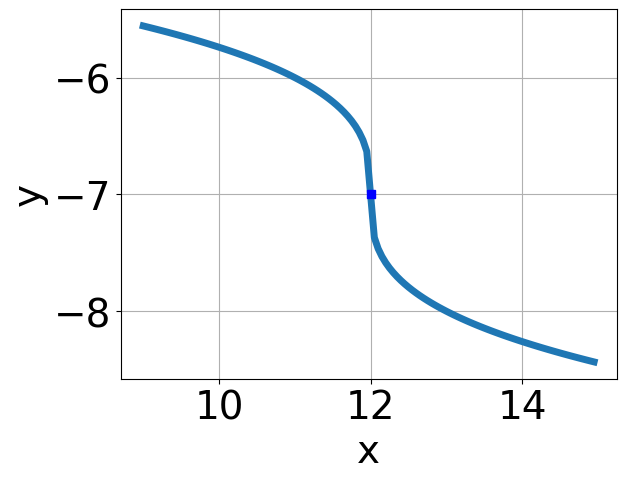
\includegraphics[width = 0.3\textwidth]{../Figures/radicalEquationToGraphCA.png}\item 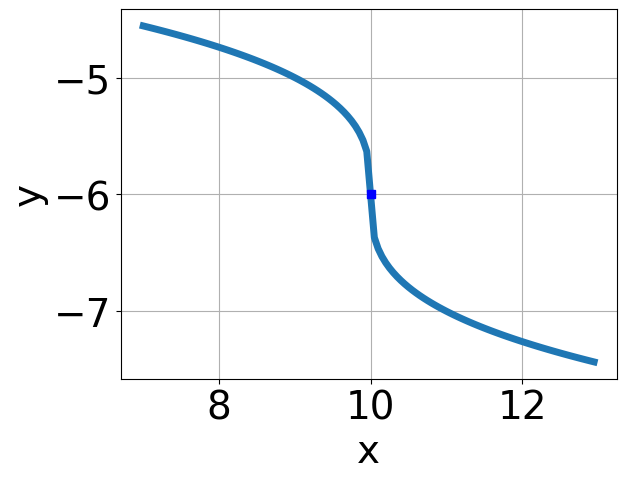
\includegraphics[width = 0.3\textwidth]{../Figures/radicalEquationToGraphDA.png}\end{multicols}\item None of the above.
\end{enumerate} }
\litem{
Choose the equation of the function graphed below.
\begin{center}
    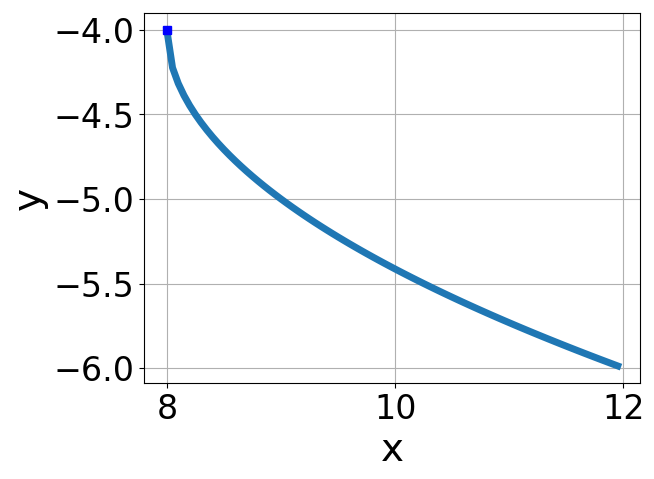
\includegraphics[width=0.5\textwidth]{../Figures/radicalGraphToEquationA.png}
\end{center}
\begin{enumerate}[label=\Alph*.]
\item \( f(x) = \sqrt[3]{x + 14} - 5 \)
\item \( f(x) = \sqrt[3]{x - 14} - 5 \)
\item \( f(x) = - \sqrt[3]{x + 14} - 5 \)
\item \( f(x) = - \sqrt[3]{x - 14} - 5 \)
\item \( \text{None of the above} \)

\end{enumerate} }
\litem{
Choose the equation of the function graphed below.
\begin{center}
    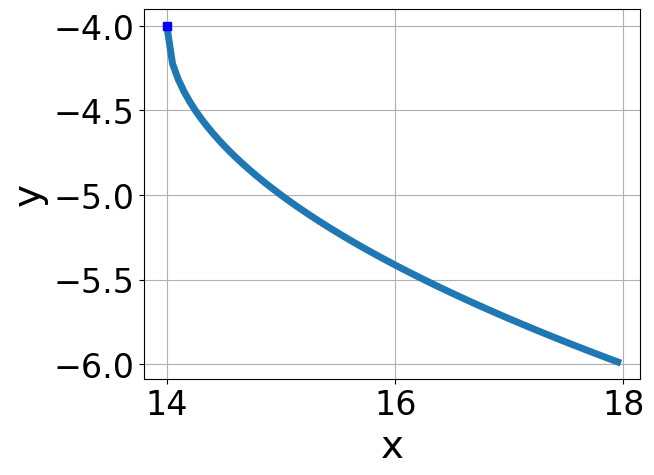
\includegraphics[width=0.5\textwidth]{../Figures/radicalGraphToEquationCopyA.png}
\end{center}
\begin{enumerate}[label=\Alph*.]
\item \( f(x) = \sqrt[3]{x + 12} - 5 \)
\item \( f(x) = - \sqrt[3]{x + 12} - 5 \)
\item \( f(x) = - \sqrt[3]{x - 12} - 5 \)
\item \( f(x) = \sqrt[3]{x - 12} - 5 \)
\item \( \text{None of the above} \)

\end{enumerate} }
\litem{
Solve the radical equation below. Then, choose the interval(s) that the solution(s) belongs to.\[ \sqrt{8 x - 2} - \sqrt{6 x + 2} = 0 \]\begin{enumerate}[label=\Alph*.]
\item \( x_1 \in [-0.66, -0.14] \text{ and } x_2 \in [0,1.3] \)
\item \( x \in [-0.19,0.13] \)
\item \( \text{All solutions lead to invalid or complex values in the equation.} \)
\item \( x_1 \in [0.06, 0.62] \text{ and } x_2 \in [1.5,3.2] \)
\item \( x \in [1.83,2.24] \)

\end{enumerate} }
\litem{
What is the domain of the function below?\[ f(x) = \sqrt[4]{8 x - 5} \]\begin{enumerate}[label=\Alph*.]
\item \( [a, \infty), \text{ where } a \in [-1.2, 0.8] \)
\item \( (-\infty, \infty) \)
\item \( (-\infty, a], \text{where } a \in [-0.8, 1.1] \)
\item \( [a, \infty), \text{where } a \in [1.1, 4.8] \)
\item \( (-\infty, a], \text{where } a \in [1.5, 2.9] \)

\end{enumerate} }
\litem{
What is the domain of the function below?\[ f(x) = \sqrt[5]{7 x + 4} \]\begin{enumerate}[label=\Alph*.]
\item \( \text{The domain is } [a, \infty), \text{   where } a \in [-4.75, -0.75] \)
\item \( \text{The domain is } [a, \infty), \text{   where } a \in [-1.57, 2.43] \)
\item \( \text{The domain is } (-\infty, a], \text{   where } a \in [-2.6, -0.7] \)
\item \( \text{The domain is } (-\infty, a], \text{   where } a \in [-1.2, -0.4] \)
\item \( (-\infty, \infty) \)

\end{enumerate} }
\litem{
Solve the radical equation below. Then, choose the interval(s) that the solution(s) belongs to.\[ \sqrt{12 x^2 - 28} - \sqrt{5 x} = 0 \]\begin{enumerate}[label=\Alph*.]
\item \( x_1 \in [0.7, 1.7] \text{ and } x_2 \in [-5.25,2.75] \)
\item \( \text{All solutions lead to invalid or complex values in the equation.} \)
\item \( x \in [1.6,2.7] \)
\item \( x \in [-2.1,-0.6] \)
\item \( x_1 \in [-2.1, -0.6] \text{ and } x_2 \in [-5.25,2.75] \)

\end{enumerate} }
\litem{
Choose the graph of the equation below.\[ f(x) = \sqrt[3]{x - 8} - 5 \]\begin{enumerate}[label=\Alph*.]
\begin{multicols}{2}\item 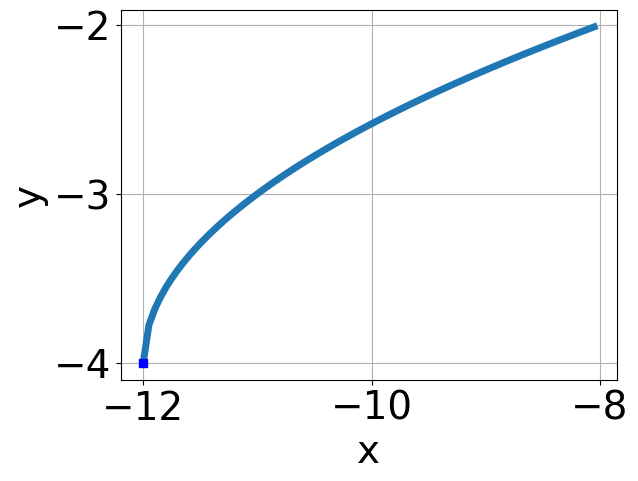
\includegraphics[width = 0.3\textwidth]{../Figures/radicalEquationToGraphCopyAA.png}\item 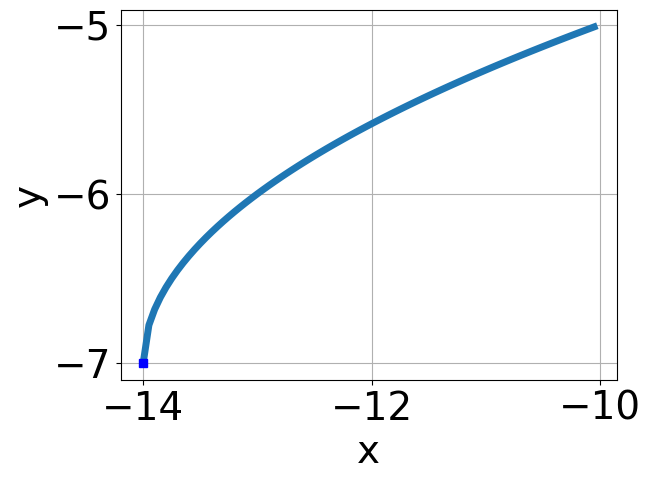
\includegraphics[width = 0.3\textwidth]{../Figures/radicalEquationToGraphCopyBA.png}\item 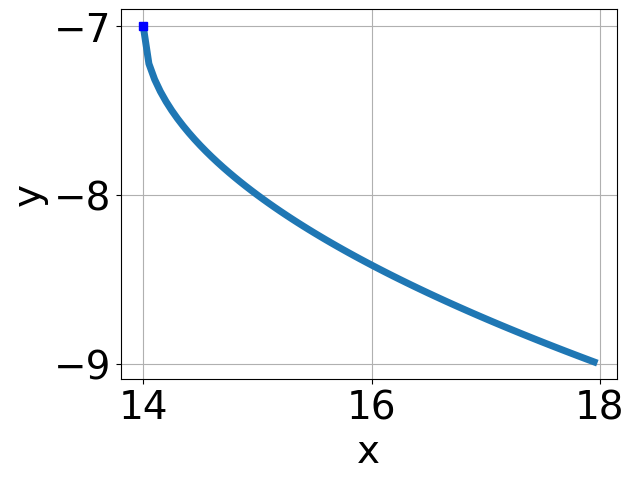
\includegraphics[width = 0.3\textwidth]{../Figures/radicalEquationToGraphCopyCA.png}\item 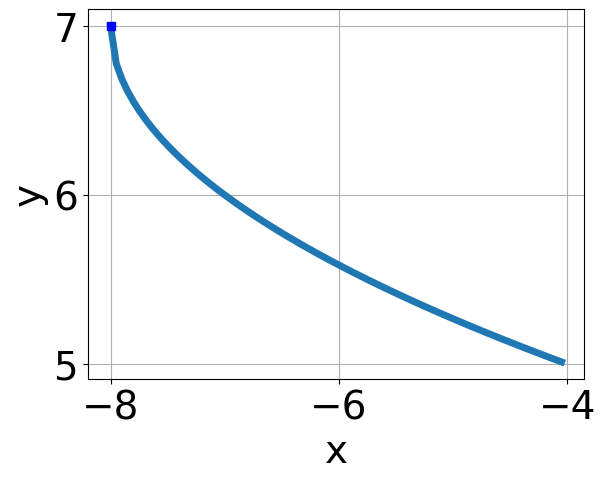
\includegraphics[width = 0.3\textwidth]{../Figures/radicalEquationToGraphCopyDA.png}\end{multicols}\item None of the above.
\end{enumerate} }
\end{enumerate}

\end{document}